\subsection{Outline the origin of the hyperfine structure. What are the assumptions made for the nucleus? Discuss the resulting splitting of the energy states.}


Ligesom elektronen har protonerne og neutronerne i kernen også et spin, da alle elementarpartikler har dette, og der tages nu højde for, at kernen også har et spin, kaldet \emph{kerneimpulsmoment} $I$ (eng. nuclear angular momentum). Som andre impulsmomenter giver kerneimpulsmomentet anledning til et magnetisk dipolmoment
\begin{align} \label{eq:Q16_NuclearAngularMomentumMagneticMoment}
	\vec{\mu}_I &= g_N \frac{\mu_N}{\hbar} \vec{I} \: ,
\end{align}
hvor der, modsat elektronens dipolmoment, ikke er et negativt fortegn, da dette stammer fra elektrones ladning\footnote{Hvis masse og ladning er fordelt identisk, så er faktoren $\gamma$ ($\vec{\mu} = \gamma \vec{L}$ for et impulsmoment $\vec{L}$) givet som $\frac{q}{2m}$, hvor $q$ er partiklens ladning og $m$ dens masse.}. I \cref{eq:Q16_NuclearAngularMomentumMagneticMoment} er $\mu_N = e\hbar/(Zm_p)$ kernemagnetronen (eng. nuclear magnetron). Kernen har et meget mindre dipolmoment end elektronerne, da kernemagnetronen er meget mindre end Bohrmagnetronen\footnote{Bohrmagnetronen er givet ved $\mu_B = \frac{e\hbar}{4m_e}$.}
\begin{align}
	\mu_B &= \frac{m_p}{m_e}\mu_N = 1836 \mu_N \: .
\end{align}

Af denne grund kan $H_{HFS}$ ses som en perturbation, og denne beregnes ved
\begin{align} \label{eq:Q16_HyperFineStructureHamiltonStart}
	H_{HFS} &= -\vec{\mu}_I \cdot \vec{B}_J
	= -\left(g_N \frac{\mu_N}{\hbar} \vec{I}\right) \cdot \left(-B_J \frac{\vec{J}}{\abs{\vec{J} \: }}\right)
	= g_N \frac{\mu_N}{\hbar} B_J \frac{\vec{I} \cdot \vec{J}}{\abs{\vec{J} \: }} \: ,
\end{align}
hvor det er benyttet, at det magnetiske felt dannet af elektronen $\vec{B}_J = - B_J \vec{J}/|\vec{J}|$, hvor fortegnet kommer fra, at vi har beregnet det magnetiske felt ved kernes position, som er $-\vec{r}$ set fra elektronens synspunkt. Et magnetisk felt i $\vec{J}$-retnignen skyldes, at vi i vektormodellen vil se en hurtig præcision omkring $\vec{J}$, og derfor vil enhver anden komponent end dem langs med $\vec{J}$ tidsgennemsnitlig være $0$ (vi lader altså det magnetiske felt projiceres ind på $\vec{J}$)\footnote{Larmorpræcisionen?}. Hermed kan energiskiftet grundet hyperfinstrukturen beregnes som
\begin{align} \label{eq:Q16_HyperFineStructureEnergyChangeStart}
    E_{HFS} &= \braket{H_{HFS}} = g_N \frac{\mu_N}{\hbar} B_J \braket{\frac{\vec{I} \cdot \vec{J}}{\abs{\vec{J} \: }}} \: .
\end{align}

Vi skifter nu basis til det totale atomarimpulsmoment $\vec{F} = \vec{I} + \vec{J}$, da kerneimpulsmomentet og det totale elektronimpulsmoment er koblede. Fra dette kan vi nu finde $\braket{\vec{I} \cdot \vec{J} \:}$
\begin{align}
    \Vec{F}^2 &= \Vec{I}^2 + \Vec{J}^2 + 2\Vec{I} \cdot \Vec{J} \nonumber\\
    \Rightarrow \braket{\Vec{I} \cdot \Vec{J}} &= \frac{1}{2} \left(\braket{\Vec{F}^2} - \braket{\Vec{I}^2} - \braket{\Vec{J}^2}\right) = \frac{\hbar^2}{2} \left\{F(F+1) - I(I+1) - J(J+1)\right\} \: ,
\end{align}
og vi ved, at $\braket{|\vec{J}|} = \hbar \sqrt{J(J+1)}$, hvorfor energiskiftet i \cref{eq:Q16_HyperFineStructureEnergyChangeStart} bliver til
\begin{align} \label{eq:Q16_HyperFineStructureEnergyChange}
    E_{HFS} &= g_N \frac{\mu_N}{\hbar} B_J \frac{\hbar^2}{2\hbar} \frac{F(F+1) - I(I+1) - J(J+1)}{\sqrt{J(J+1)}} \nonumber\\
    &= \frac{A}{2}\left\{F(F+1) - I(I+1) - J(J+1)\right\} \: , \quad \text{hvor} \quad A = \frac{g_N \mu_N B_J}{\sqrt{J(J+1)}} \: .
\end{align}
Her er $A$ \emph{hyperfinstrukturkonstanten} og det resterende kaldes \emph{intervalfaktoren}. \textbf{Note:} I $B_J$ er Bohrmagnetronen $\mu_B$ indeholdt.


\paragraph{Opsplitning:} Hyperfinstrukturen vil dermed give en opsplitning til $F$-tilstande, hvorfor udartetheden (eng. degeneracy) i $J$ løftes.\\

Som eksempel kan vi se på 2P-tilstanden i hydrogen. Her er $n = 2$ og $l = 1$, og siden at vi taler om en enkelt elektron vil $s = 1/2$, hvorfor $j = 1/2,\: 3/2$. Hydrogenkernen består af en enkelt proton, hvilken har spin $1/2$, hvorfor $I = 1/2$. Derved bliver $F = 1,\: 2$ og $F = 0,\: 1$ hhv.. Dette kan ses af \cref{fig:Q16_HyperFineSplittingOf2PstateInHydrogen}.
\begin{figure}[!h]
    \centering
    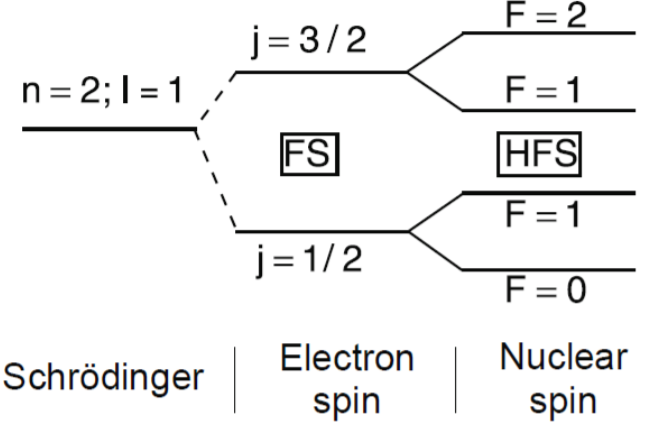
\includegraphics[width=0.60\textwidth]{Q16/images/HyperFineSplittingOf2PstateInHydrogen.PNG}
    \caption{Fin- og hyperfinstrukturopsplitning af 2P-tilstanden i hydrogen. $n = 2$, $l = 1$, så $j = \frac{1}{2}, \: \frac{3}{2}$ og $F = 0,\: 1,\: 2$. Not to scale.}
    \label{fig:Q16_HyperFineSplittingOf2PstateInHydrogen}
\end{figure}\\
Energiskiftet grundet finstrukturen vil dermed for $F = 2$ (og $j = \frac{3}{2}$) tilstanden være
\begin{align}
    E_{HFS} &= \frac{A}{2} \left\{F(F+1) - I(I+1) - J(J+1)\right\} \nonumber\\
    &= \frac{A}{2} \left\{2(2+1) - \frac{3}{2}(\frac{3}{2}+1) - \frac{1}{2}(\frac{1}{2}+1)\right\} \nonumber\\
    &= \frac{A}{2} \left\{2 \cdot 3 - \frac{3}{2} \cdot \frac{5}{2} - \frac{1}{2} \cdot \frac{3}{2}\right\} \nonumber\\
    &= \frac{A}{2} \left\{6 - \frac{15}{4} - \frac{3}{4}\right\} \nonumber\\
    &= \frac{A}{2} \left\{\frac{24}{4} - \frac{18}{4}\right\}
    = \frac{A}{2} \left\{\frac{6}{4}\right\} \nonumber\\
    &= \frac{3A}{4} \: .
\end{align}
For $F = 1$ (og $j = \frac{3}{2}$) tilstanden vil energiskiftet være
\begin{align}
    E_{HFS} &= \frac{A}{2} \left\{F(F+1) - I(I+1) - J(J+1)\right\} \nonumber\\
    &= \frac{A}{2} \left\{1(1+1) - \frac{3}{2}(\frac{3}{2}+1) - \frac{1}{2}(\frac{1}{2}+1)\right\} \nonumber\\
    &= -\frac{5A}{4} \: .
\end{align}
Dette overholder \emph{intervalreglen}
\begin{align}
    (E_{HFS})_F - (E_{HFS})_{F-1} &= FA \: ,
\end{align}
hvilket overholdes, da
\begin{align}
    (E_{HFS})_2 - (E_{HFS})_1 &= \frac{3A}{4} - \left(-\frac{5A}{4}\right) = \frac{3A}{4} + \frac{5A}{4} = 2A \: .
\end{align}